%%%%%%%%%%%%%%%%%%%%%%%%%%%%%%%%%%%%%%%%%%%%%%%%%%%%%%%%%%%%%%%%%%%%%%%%%%%%%%%%
% Alarm
%%%%%%%%%%%%%%%%%%%%%%%%%%%%%%%%%%%%%%%%%%%%%%%%%%%%%%%%%%%%%%%%%%%%%%%%%%%%%%%%
\chapter{Alarm} \label{Alarm}
\vspace{-10ex}\mAl{syml}\vskip 8ex

%%%%%%%%%%%%%%%%%%%%%%%%%%%%%%%%%%%%%%%%%%%%%%%%%%%%%%%%%%%%%%%%%%%%%%%%%%%%%%%%
% Introduction
%%%%%%%%%%%%%%%%%%%%%%%%%%%%%%%%%%%%%%%%%%%%%%%%%%%%%%%%%%%%%%%%%%%%%%%%%%%%%%%%
\section{Introduction}

The \mAl{f} is a \textit{time of day} alarm.  It runs independent of any mode
and can wake the device from any power state.  Both the \cBe{f} and \mAu{f}
can be used as wakeup sources.  Refer to \hyperref[Set Alarm]{\mSA{f}}
for configuration.

%%%%%%%%%%%%%%%%%%%%%%%%%%%%%%%%%%%%%%%%%%%%%%%%%%%%%%%%%%%%%%%%%%%%%%%%%%%%%%%%
% Disabled
%%%%%%%%%%%%%%%%%%%%%%%%%%%%%%%%%%%%%%%%%%%%%%%%%%%%%%%%%%%%%%%%%%%%%%%%%%%%%%%%
\section{Disabled} \label{Alarm - Disabled} \sAlDi{syml}

If the alarm is \sAlDi{f}, it will stay in the \sAlDi{f} state until enabled
via \hyperref[Set Alarm]{\mSA{f}}.

%%%%%%%%%%%%%%%%%%%%%%%%%%%%%%%%%%%%%%%%%%%%%%%%%%%%%%%%%%%%%%%%%%%%%%%%%%%%%%%%
% Off
%%%%%%%%%%%%%%%%%%%%%%%%%%%%%%%%%%%%%%%%%%%%%%%%%%%%%%%%%%%%%%%%%%%%%%%%%%%%%%%%
\section{Off} \label{Alarm - Off} \sAlOf{syml}

This is the initial and final state if the alarm is enabled.  When the current
time equals the alarm time, the alarm will start, and either

\begin{enumerate}
  \item Start playing an \mAu{f} track, \textit{or}
  \item Start alerting with the \cBe{f}
\end{enumerate}

depending on which was configured in \hyperref[Set Alarm]{\mSA{f}}. It will then
enter the \sAlWa{f} state.

\as{{c c c c}}{\sAlOf{sym} & \aTi{sym} & \eStart{sym}{ALARM} & \sAlWa{sym} \\}

\info{If a track is currently playing when the alarm starts, the beeper will be
used regardless of setting - this is so you know that the alarm has started.}

%%%%%%%%%%%%%%%%%%%%%%%%%%%%%%%%%%%%%%%%%%%%%%%%%%%%%%%%%%%%%%%%%%%%%%%%%%%%%%%%
% Wake
%%%%%%%%%%%%%%%%%%%%%%%%%%%%%%%%%%%%%%%%%%%%%%%%%%%%%%%%%%%%%%%%%%%%%%%%%%%%%%%%
\section{Wake} \label{Alarm - Wake} \sAlWa{syml}

In this state, the \cBe{f} will alert or the \mAu{f} will play a track.  To
\sAlSn{f} the alarm, do one of the following:

\begin{itemize}
  \item \aTo{f} the \dTo{f} of the enclosure.\footnote{ This assumes that touch
    has been enabled via \hyperref[Touch Settings]{\mTS{ss}}.}
  \item \aTu{f} the \cEs{f}.
\end{itemize}

\as{{c c c c}}{%
\multirow{2}{*}{\sAlWa{sym}} & \sTo
  & \multirow{2}{*}{\eSnooze{sym}{ALARM}}
  & \multirow{2}{*}{\sAlSn{sym}} \\ \dcrule{2}{2}
& \sTu & & \\}

The \cDi{f} will show

\begin{figure}[H]
\centering
  \sDl{Snoo}
\end{figure}

when either of the two above actions are taken.

\par\medskip

If a \sSAWT{f} has been configured and the alarm has been in the \sAlWa{f}
state for longer than that time, the alarm will stop, reset for the next day
and go to the \sAlOf{f} state.

\as{{c c c c}}{\sAlWa{sym} & \aWT{sym} & \eSt{sym}{ALARM} & \sAlOf{sym} \\}

%%%%%%%%%%%%%%%%%%%%%%%%%%%%%%%%%%%%%%%%%%%%%%%%%%%%%%%%%%%%%%%%%%%%%%%%%%%%%%%%
% Snooze
%%%%%%%%%%%%%%%%%%%%%%%%%%%%%%%%%%%%%%%%%%%%%%%%%%%%%%%%%%%%%%%%%%%%%%%%%%%%%%%%
\section{Snooze} \label{Alarm - Snooze} \sAlSn{syml}

The \mAu{f} will be paused or the \cBe{f} will stop when the alarm is snoozed.
It will resume when the configured \sSAST{f} has elapsed.

\as{{c c c c}}{\sAlSn{sym} & \aST{sym} & \eResume{sym}{ALARM} & \sAlWa{sym} \\}

%%%%%%%%%%%%%%%%%%%%%%%%%%%%%%%%%%%%%%%%%%%%%%%%%%%%%%%%%%%%%%%%%%%%%%%%%%%%%%%%
% In Progress
%%%%%%%%%%%%%%%%%%%%%%%%%%%%%%%%%%%%%%%%%%%%%%%%%%%%%%%%%%%%%%%%%%%%%%%%%%%%%%%%
\section{In Progress} \label{Alarm - In Progress} \sAlIP{syml}

This includes both the \sAlWa{f} and \sAlSn{f} states.  To stop the alarm,
\aPR{f} the \cEs{f}.

\par\medskip

The \cDi{f} will show

\begin{figure}[H]
\centering
  \sDl{OFF!}
\end{figure}

when the above action is taken.

\as{{c c c c}}{\sAlIP{sym} & \sPR & \eSt{sym}{ALARM} & \sAlOf{sym} \\}

If a \sSATT{f} has been configured and the alarm has been \sAlIP{f} for
more than this time, it will turn off and go to the \sAlOf{f} state.

\as{{c c c c}}{\sAlIP{sym} & \aTT{sym} & \eSt{sym}{ALARM} & \sAlOf{sym} \\}

In either case, the alarm will automatically reset for the next day.

%%%%%%%%%%%%%%%%%%%%%%%%%%%%%%%%%%%%%%%%%%%%%%%%%%%%%%%%%%%%%%%%%%%%%%%%%%%%%%%%
% Reference
%%%%%%%%%%%%%%%%%%%%%%%%%%%%%%%%%%%%%%%%%%%%%%%%%%%%%%%%%%%%%%%%%%%%%%%%%%%%%%%%
\section{Reference} \label{Alarm - Reference}

\ers{2}
\begin{longtabu}{ X[2,c,m] | X[2,c,m] | X[3,c,m] | X[2,c,m] }
  \thrule
  \thbi{State} & \thbi{Action} & \thbi{Effect} & \thbi{Next} \\ \mrule

  \sAlDi{sym} & --- & --- & --- \\ \mrule

  \sAlOf{sym} & \fontTGA{ss}{TIME = ALARM TIME}
    & \eStart{sym}{ALARM} & \sAlWa{sym} \\ \mrule

  \multirow{5}{*}[-1.5mm]{\sAlWa{sym}}
    & \sTo & \multirow{2}{*}[-1mm]{\eSnooze{sym}{ALARM}}
    & \multirow{2}{*}[-1mm]{\sAlSn{sym}} \\ \dcrule{2}{2}
  & \sTu & & \\ \dcrule{2}{4}
  & \sPR & & \\ \dcrule{2}{2}
  & \fontTGA{ss}{WAKE TIME EXCEEDED}
    & \eSt{sym}{ALARM} & \sAlOf{sym} \\ \dcrule{2}{2}
  & \fontTGA{ss}{TOTAL ALARM TIME EXCEEDED} & & \\ \mrule

  & \fontTGA{ss}{SNOOZE TIME EXPIRED}
    & \eWake{sym}{ALARM} & \sAlWa{sym} \\ \dcrule{2}{4}

  \sAlSn{sym} & \sPR
    & \multirow{2}{*}[-1mm]{\eSt{sym}{ALARM}}
    & \multirow{2}{*}[-1mm]{\sAlOf{sym}} \\ \dcrule{2}{2}

  & \fontTGA{ss}{TOTAL ALARM TIME EXCEEDED} & & \\

  \bhrule
\caption{Alarm - Reference}
\end{longtabu}

%%%%%%%%%%%%%%%%%%%%%%%%%%%%%%%%%%%%%%%%%%%%%%%%%%%%%%%%%%%%%%%%%%%%%%%%%%%%%%%%
% State Diagram
%%%%%%%%%%%%%%%%%%%%%%%%%%%%%%%%%%%%%%%%%%%%%%%%%%%%%%%%%%%%%%%%%%%%%%%%%%%%%%%%
\section{State Diagram} \label{Alarm - State Diagram}

\begin{figure}[H]
\centering
  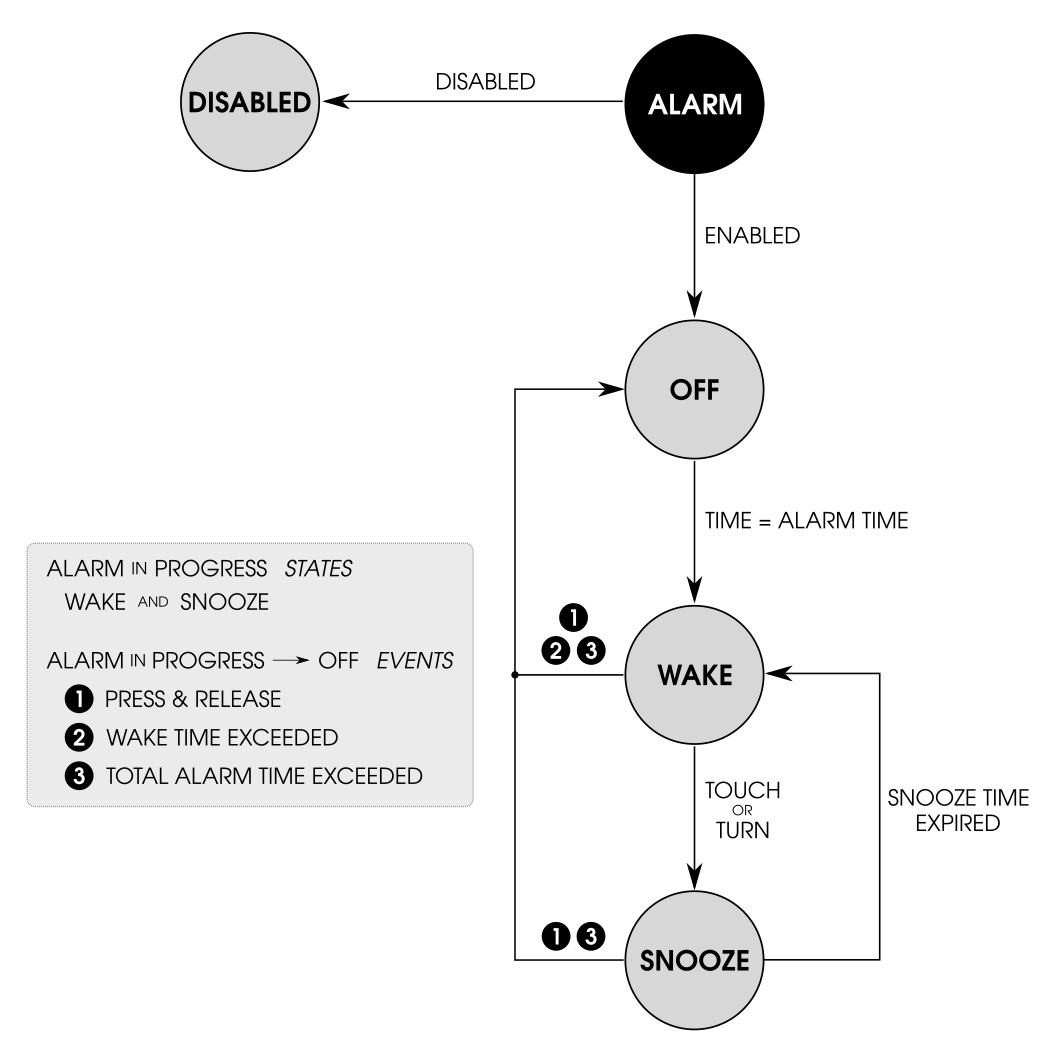
\includegraphics{images/alarm_state_diagram.png}
\caption{Alarm - State Diagram}
\end{figure}
